%% PROPOSAL: Generation of elliptic curves for circuit use.
%% Marta, Barry and Jordi.
%% The 2nd ZKProof Workshop 2019.

\documentclass{article}

% Packages
	\usepackage[colorlinks=true,
				urlcolor=black,
				linkcolor=black,
				citecolor=black
				]{hyperref} 
	
	\usepackage[english]{babel}
	\usepackage[utf8]{inputenc}
	\usepackage{amsmath, amsthm, amssymb, mathtools}
	\usepackage{enumerate, enumitem}
	\usepackage{graphicx, color, xcolor}
	\usepackage{setspace}
	\usepackage{authblk}
	\usepackage{braket}
	
	\usepackage{algorithm}
	\usepackage[noend]{algpseudocode}
	\makeatletter
	\def\BState{\State\hskip-\ALG@thistlm}
	\makeatother
	
	\usepackage{listings}
	\lstdefinelanguage{Sage}[]{Python}
	{morekeywords={False,sage,True},sensitive=true}
	\lstset{frame=none,
			showtabs=False,
			showspaces=False,
			showstringspaces=False,
			commentstyle={\ttfamily\color{dgreencolor}},
			keywordstyle={\ttfamily\color{dbluecolor}\bfseries},
			stringstyle={\ttfamily\color{dgraycolor}\bfseries},
			language=Sage,
			basicstyle={\fontsize{10pt}{10pt}\ttfamily},
			aboveskip=0.3em,
			belowskip=0.1em,
			numbers=none,%left,
			numberstyle=\footnotesize
			}
		
	\definecolor{dblackcolor}{rgb}{0.0,0.0,0.0}
	\definecolor{dbluecolor}{rgb}{0.01,0.02,0.7}
	\definecolor{dgreencolor}{rgb}{0.2,0.4,0.0}
	\definecolor{dgraycolor}{rgb}{0.30,0.3,0.30}
	\newcommand{\dblue}{\color{dbluecolor}\bf}
	\newcommand{\dred}{\color{dredcolor}\bf}
	\newcommand{\dblack}{\color{dblackcolor}\bf}

% Commands	
	\newcommand{\N}{\ensuremath{\mathbb{N}}}
	\newcommand{\Np}{\ensuremath{\mathbb{N}^{+}}}
	\newcommand{\Z}{\ensuremath{\mathbb{Z}}}
	\newcommand{\Q}{\ensuremath{\mathbb{Q}}}
	\newcommand{\R}{\ensuremath{\mathbb{R}}}
	\newcommand{\C}{\ensuremath{\mathbb{C}}}
	\newcommand{\Fp}{\ensuremath{\mathbb{F}_p}}
	\newcommand{\Fr}{\ensuremath{\mathbb{F}_r}}
	\newcommand{\G}{\ensuremath{\mathbb{G}}}
	\newcommand{\point}[1]{P_{#1} = (x_{#1}, y_{#1})}
	\newcommand{\llog}{\log_2}
	\newcommand{\xor}{\oplus}
	\newcommand{\minSize}{1.5em}
	\newcommand{\gen}[1]{\ensuremath{\langle #1\rangle}}
	\newcommand{\noi}{\noindent}
	\newcommand{\red}[1]{\textcolor{red}{#1}}
	\newcommand{\blue}[1]{\textcolor{blue}{#1}}

% Margins
	\textwidth 16 cm
	\textheight 23.5 cm
	\topmargin -1.5 cm
	\oddsidemargin -0 cm
	
	\addtolength{\skip\footins}{1pc plus 5pt} % Foot note space
	\setlength\parindent{0pt} % No indent

% Title
	\makeatletter
	\renewcommand\AB@affilsepx{, \protect\Affilfont}
	\makeatother

	\title{Generation of (Twisted Edwards) elliptic curves for circuit use 
			\vspace{-0.2cm} }
	\author[1]{Barry WhiteHat}
	\author[2]{Jordi Baylina}
	\author[2,3]{Marta Bellés}
	\affil[1]{Ethereum foundation}
	\affil[2]{iden3}
	\affil[3]{Universitat Pompeu Fabra}
	\setcounter{Maxaffil}{0}
	\renewcommand\Affilfont{\itshape\small}

\begin{document}
\begin{spacing}{1.2}	

\maketitle  	  \vspace{1.5cm}
\tableofcontents  \vspace{0.5cm}


\newpage

%%
\section{Scope, motivation and background}
	
	Motivation:
	\begin{itemize}
		\item 	Protocols like zk-SNARK require the usage of pairing-friendly elliptic curves (references to SNARK, pairing-friendly elliptic curves and BN, BL).
		\item 	What happens if inside the circuit we need to implement protocols that use elliptic curves, such as Pedersen Hash and EdDSA. 
		\item 	Inside the SNARK, we have elements of a certain field $\Fp$ (which is the order of the pairing-friendly curve, is at always of prime order?)
		\item 	So, we have to find what we call an {\it embedded curve} defined over $\Fp$.
	\end{itemize}
	
	Aim:
	\begin{itemize}
		\item 	This proposal aims to define a deterministic algorithm for generating elliptic curves defined over a given prime field. 
				That is, given a prime $p$, generate an elliptic curve defined over $\Fp$.
		\item 	It is important the ability to find it in a deterministic way---so that it was clear no other considerations were taken for defining---is 
				paramount as it significantly reduces the possibility of a backdoor being present, thus leading to better security.
		\item 	Also: provide an algorithm for checking its safety against best known attacks. 
		\item 	We present an example of a generated curve done this way: Baby Jubjub. Also include the arithmetic implementation of it. 
	\end{itemize}

	Background:
	\begin{itemize}
		\item Elliptic curve? Pairing-friendly (BN, BL)? Twisted Edwards / Montgomery elliptic curve? (Add REF).
		\item Order of the elliptic curve? Large prime dividing the order?
		\item Safety criteria: add attacks? (Add REF?)
	\end{itemize}
	
	Terminology:
	\begin{itemize}
		\item {\it Embedded elliptic curve}: given an elliptic curve $E$ of prime order $p$, an elliptic curve $E'$ defined over $\Fp$ is called an embedded elliptic curve of $E$. 
	\end{itemize}

	Notation:
	\begin {table}[h!]
		\centering
		\begin{tabular}{|c|l|}
			\hline
			{\bf Notation} 	& {\bf Description} \\ 
			\hline
			{$E$} 			& Twisted Edwards elliptic curve.\\ 
			\hline		
			{$p$} 			& Prime number. Characteristic of the field $E$ is defined over.\\ 
			\hline
			\begin{tabular}{@{}c@{}}	{$a$}  \\ {$d$} \end{tabular}
				  			& Parameters of the equation $ax^2 + y^2 = 1 +  d x^2 y^2$.\\ \hline
			{$n$} 			& Order of the curve. Typically, $n = h\times l$. \\ 
			\hline
			{$l$} 			& Large prime dividing the order of the curve.\\ 
			\hline
			{$h$} 			& Cofactor.\\ 
			\hline
			{$x_0, y_0$} 	& Generator of the curve.\\ 
			\hline
			{$x_1, y_1$} 	& Generator of the large prime subgroup of the curve.\\ 
			\hline
		\end{tabular}
		\label{tab:notation}
	\end{table}

%%
\section{Generation of embedded elliptic curves}
	Definition of the curve:
	\begin{itemize}
		\item Finite field (defined by $p$).
		\item Order of the curve and its prime decomposition* (in case of TEd/Mont: cofactor and large prime).
		\item Generator and base point.
	\end{itemize}
	
	%%
	\subsection{Twisted Edwards and Montgomery}
	%TODO: Write and justify the assumptions.
				
		In 2016, a group of researchers of IRPF designed a deterministic algorithm that, given a prime number $p$, it returns the elliptic curve defined over $\Fp$ with smallest coefficient $A$ such that $A-2$ is a multiple of 4 and equation $y^2 = x^3 + Ax^2 + x$ describes a Montgomery curve. 
		The assumption $A-2$ divisible by 4 comes from the fact that as this value is used in many operations, so trying to keep it smaller and divisible by four is a reasonable assumption \cite{generation-baby}.
		
		\subsubsection{Generation of elliptic curves given $p$ with $p\equiv1\mod4$} \begin{lstlisting}
import sys
import pdb

def findCurve(prime, curveCofactor, twistCofactor, _A):
	F = GF(prime)
	A = _A
	while A < _A + 100000:
		print A
		if (A-2.) % 4 != 0:
			A+=1.
			continue
		try:
			E = EllipticCurve(F, [0, A, 0, 1, 0])
		except:
			A+=1.
			continue
		groupOrder = E.order()
		if (groupOrder % curveCofactor != 0
		or not is_prime(groupOrder // curveCofactor)):
			A+=1
			continue

		twistOrder = 2*(prime+1)-groupOrder
		if (twistOrder % twistCofactor != 0
		or not is_prime(twistOrder // twistCofactor)):
			A+=1
			continue
		return A, E

def find1Mod4(prime, curveCofactor, twistCofactor, A):
	assert((prime % 4) == 1)
	return findCurve(prime, curveCofactor, twistCofactor, A)

def findGenPoint(prime, A, EC, N):
	F = GF(prime)
	for uInt in range(1, 1e3):
		u = F(uInt)
		v2 = u^3 + A*u^2 + u
		if not v2.is_square():
			continue
		v = v2.sqrt()
	
		point = EC(u, v)
		pointOrder = point.order()
		if pointOrder == N:
			return point

def mont_to_ted(u, v , r):
	x = Mod(u / v, r) 
	y = Mod((u-1)/(u+1), r) 
	return(x, y)

def ted_to_mont(x, y , r):
	u = Mod((1 + y )/ ( 1 - y)  , r)
	v = Mod((1 + y ) / ( (1 - y) * x) , r ) 
	return(u,v)

def isOnEd(x,y,r,a,d):
	return Mod(Mod(a,r)*(x**2),r) + Mod(y**2 , r) - 1 
	- Mod(d,r)*(Mod(x**2,r))*(Mod(y**2,r)) == 0 
\end{lstlisting}
\vspace{0.5cm}
				
		\subsubsection{Generation of elliptic curves given $p$ with $p\equiv3\mod4$}
		%TODO: Add text
		
	%% 
	%TODO
	\subsection{Elliptic curves of prime order}
	\subsection{Pairing-friendly elliptic curves}

%%
\section{Safety criteria}
	% TODO
	SafeCurves is a project that checks some of the most common and known attacks on several elliptic curves. It also provides the algorithm it was used \cite{safe-curves}.
	
	\begin{itemize}
		\item 
	\end{itemize}

%%
\section{Example: embedded curve of BN128 generation of Baby Jubjub}
	
	%%
	\subsection{Generation Of Baby Jubjub}
		We considered the large prime number dividing the order of BN128 and run algorithm A.1 from \cite{generation-baby}. The first elliptic curve it was returned  satisfying SafeCurves criteria was the Montgomery curve with coefficient $A = 168698$. We named this curve Baby Jubjub elliptic curve. 

		\subsubsection{Code}
		\begin{lstlisting}
prime = 218882428718392752222464057452572750885
	48364400416034343698204186575808495617
Fr = GF(prime)
h = 8 # cofactor

A = int(sys.argv[1])
A, EC = find1Mod4(prime, h, 4, A)

# A = 170214 another candidate
B = 1
a = A + 2 / B
d = A - 2 / B

print "a " , a , "d " , d , sqrt(d)
# check we have a safe twist
assert(not d.is_square())
assert(a*d*(a-d)!=0)

s = factor(EC.order())
print ("l : " , s)
N = h * s # order of the curve
print (factor(EC.quadratic_twist().order()))

# get generator point
u_gen, v_gen, w_gen = findGenPoint(prime, A, EC, N)
# find that generator point on the edwards curve
gen_x, gen_y = mont_to_ted(u_gen, v_gen, prime)
# make sure the generator point is on the twisted edwards curve
assert(isOnEd(gen_x, gen_y, prime, a , d))
# go back to montgomery
u , v = ted_to_mont(gen_x, gen_y, prime)
# confirm we are back where we started from
assert (u == u_gen)
assert (v == v_gen)

# get base point on montgorery curve by multiplying the generator point by h
base_x , base_y, base_z = h*EC(u_gen, v_gen)
# find the same points on twisted edwards curve
base_x , base_y = mont_to_ted(base_x , base_y, prime)

# the generator is on the twisted edwards curve
assert(isOnEd(base_x,base_y, prime , a , d))

print ("generator :" , gen_x, gen_y)
print ("base :", base_x, base_y)
\end{lstlisting}\vspace{0.5cm}

	%%
	\subsection{Definition Of Baby Jubjub}
		From now on, let 
			$$	p = 21888242871839275222246405745257275088548364
					400416034343698204186575808495617 $$
		and $\Fp$ the finite field with $p$ elements. 
		
		%%
		\subsubsection{Montgomery Form}
			We define $E_M$ as the {\it Baby-Jubjub} Montgomery elliptic curve defined over $\Fp$ given %described
			by equation
			$$	E: v^2 = u^3 +  168698u^2 + u. $$
			The order of $E_M$ is $n = 8\times l$, where 
			$$	l = 2736030358979909402780800718157159386076813972
			158567259200215660948447373041 $$ 
			is a prime number. Denote by $\G$ the subgroup of points of order $r$, that is, %of $E$ 
			$$\G = \Set{ P \in E(\Fp) | l P = O  }.$$

		%%
		\subsubsection{Edwards Form}
			$E_M$ is birationally equivalent to the Edwards elliptic curve %[REF] defined by  
				$$	E: x^2 + y^2 = 1 +  d x^2 y^2 $$
			where
			$ d = 9706598848417545097372247223557719406784115219466060233080913168975159366771.$ \\
			
			The birational equivalence \cite[Thm. 3.2]{twisted} from $E$ to $E_M$ is the map
			% These results are from \cite[Theorem 3.2]{twisted}. 
			$$ (x,y) \to (u,v) = \left( \frac{1 + y}{1 - y} , \frac{1 + y}{(1 - y)x} \right) $$
			with inverse from $E_M$ to $E$
			$$ (u, v) \to (x, y) = \left(  \frac{u}{v}, \frac{u - 1}{u + 1}   \right). $$

		%%
		\subsubsection{Parameters}
			\begin {table}[h!]
				\centering
				\begin{tabular}{|c|l|}
					\hline
					{\bf Notation} & {\bf Value}\\
					\hline
					{$p$} 	&	21888242871839275222246405745257275088548364400416034343698204186575808495617 \\
					\hline
					{$a$} 	& -1 \\
					\hline
					{$d$} 	& 12181644023421730124874158521699555681764249180949974110617291017600649128846 \\
					\hline
					{$n$} 	& 21888242871839275222246405745257275088614511777268538073601725287587578984328 \\
					\hline
					{$l$} 	& 2736030358979909402780800718157159386076813972158567259200215660948447373041 \\
					\hline
					{$h$} 	& 8 \\
					\hline
					{$x_0$} & 995203441582195749578291179787384436505546430278305826713579947235728471134 \\
					\hline
					{$y_0$} & 5472060717959818805561601436314318772137091100104008585924551046643952123905 \\
					\hline
					{$x_1$} & 5299619240641551281634865583518297030282874472190772894086521144482721001553 \\
					\hline
					{$y_1$} & 16950150798460657717958625567821834550301663161624707787222815936182638968203 \\
					\hline
				\end{tabular}
				\label{tab:baby-jubjub}
			\end{table}
	
	\subsection{Arithmetic In Baby Jubjub}
		In this section we define how to operate in the elliptic curve group: %two operations supported in the elliptic curve group: 
		the addition of points and multiplication of a point by a scalar (an element of $\Fp$).
		 	\subsubsection{Addition Of Points} When adding points of elliptic curves %usually
in Montgomery form,  
one has to be careful if the points being added are equal (doubling) or not (adding) and if one of the points is the point at infinity \cite{montgomery}. 
%
Edwards curves have the advantage that there is no such case distinction and doubling can be performed with exactly the same formula as addition \cite{twisted}. 
%
In comparison, operating in Montgomery curves is cheaper. In this section, we summarize how addition and doubling is performed in both forms. 
%
For the exact number of operations required in different forms of elliptic curves, see \cite{twisted}.

\begin{itemize}
	
	\item \underline{Edwards}: 	
	% https://eprint.iacr.org/2008/013.pdf (sec 6)
	Let $\point{1}$ and $\point{2}$ be points of the Baby-Jubjub twisted Edwards elliptic curve $E$. The sum $P_1 + P_2$ is a third point $P_3 = (x_3, y_3)$ with 
		\begin{align*}
			&\lambda = d x_1x_2y_1y_2,\\
			&x_3 = (x_1y_2 + y_1x_2) / (1 + \lambda),\\
			&y_3 = (y_1y_2 - x_1x_2) / (1 - \lambda).
		\end{align*}
	Note that the neutral element is the point $O = (0,1)$ and the inverse of a point $(x,y)$ is $(-x,y)$.

	\item \underline{Montgomery}: 
	% https://link.springer.com/content/pdf/10.1007/978-3-540-46588-1_17.pdf
	Let $\point{1}\not=O$ and $\point{2}\not=O$ be two points of the Baby-JubJub elliptic curve $E_M$ in Montgomery form. 
	
	If $P_1\not=P_2$, then the sum $P_1 + P_2$ is a third point $P_3 = (x_3, y_3)$ with coordinates
	% Addition
		\begin{align}
		\label{eq-ted}
		\begin{split}
			&\Lambda = (y_2-y_1)/ (x_2-x_1),\\
			&x_3 = \Lambda^2 - A - x_1 - x_2,\\
			&y_3 = \Lambda(x_1- x_3) - y_1.
		\end{split}
		\end{align}
	%
	If $P_1 = P_2$, then $2\cdot P_1$ is a point $P_3 = (x_3, y_3)$ with coordinates
	% Doubling:
		\begin{align}
		\label{eq-mont}
		\begin{split}
			&\Lambda = (3x_1^2 + 2Ax_1 + 1)/ (2y_1),\\
			&x_3 = \Lambda^2 - A - 2x_1,\\
			&y_3 = \Lambda(x_1- x_3) - y_1.
		\end{split}	
		\end{align}
	
\end{itemize}
		 	\subsubsection{Multiplication Of A Point Of $E$ By A Scalar} Let $P\not= O$ be a point of the Edwards curve $E$ of order strictly greater than 8 (i.e. $P\in\G$) and let $k$ a binary number representing an element of $\Fp$. We describe the circuit used to compute the point $k\cdot P$.

\begin{enumerate}
	
	\item First, we divide $k$ into chunks of 248 bits. If $k$ is not a multiple of 248, we take $j$ segments of 248 bits and leave a last chunk with the remaining bits. More precisly, write 
	% TODO: The reason we do this? Dir que $r$ són tants bits (248)?
		\begin{gather*}
		k = k_0 k_1 \dots k_j 	\quad\text{with}\quad 
			\begin{cases}
			k_i = b^i_0 b^i_1 \dots b^i_{247} 	\;\text{ for }  i = 0, \dots, j-1, \\
			k_j = b^j_0 b^j_1 \dots b^j_s 	\;\text{ with } s\leq 247.
			\end{cases}
		\end{gather*}
	Then,  
		\begin{equation}
		\label{kP}
			k\cdot P = k_0\cdot P + k_1\cdot 2^{248}P +\dots+ k_j\cdot 2^{248j}P. 	
 		\end{equation}
	This sum is done using the following circuit. 
	The terms of the sum are calculated separately inside the \textsc{seq} boxes and then added together. 

	\begin{figure}[h]
		\centering
		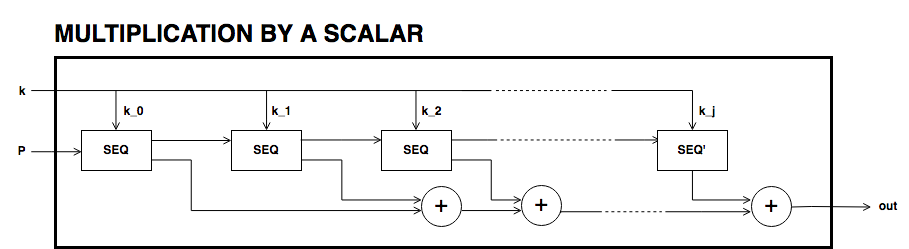
\includegraphics[scale=0.45]{figures/multiplication.png}
	\end{figure}
	
	\item Each \textsc{seq} box takes a point of $E$ of the from $P_i = 2^{248 i} P$ for $i=0,\dots,j-1$ and outputs two points %of $E$,
		$$ 	
			2^{248} \cdot P_i 
			\quad \text{and} \quad
			\sum_{n = 0}^{247} b_n \cdot 2^{n} \cdot P_i. 
		$$
	The first point is the input of the next $(i+1)$-th \textsc{seq} box (note that $ 2^{248} \cdot P_i = P_{i+1}$) whereas the second output is the computation of the $i$-th term in expression (\ref{kP}). The precise circuit is depicted in next two figures \textsc{seq} and \textsc{window}.
	
	\begin{figure}[h]
		\centering
		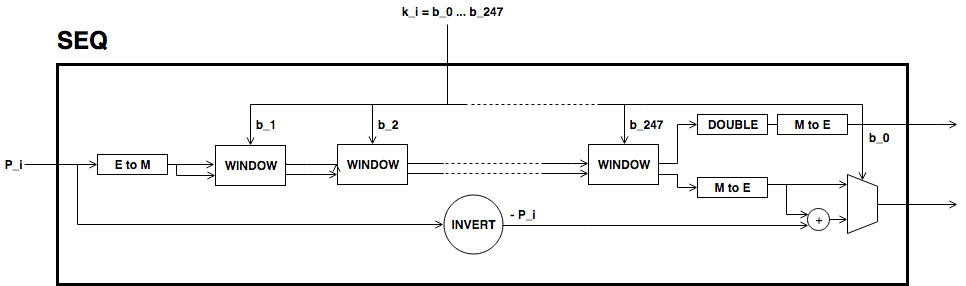
\includegraphics[scale=0.43]{figures/multiplication-SEQ.png}\\
		\vspace{0.5cm}
		
		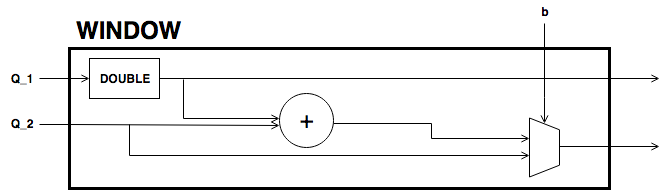
\includegraphics[scale=0.45]{figures/multiplication-SEQ-window.png}
		\vspace{0.3cm}
	\end{figure}

	The idea of the circuit is to first compute %some point 		
		$$	Q = P_i + b_1 \cdot (2P_i) + b_2 \cdot (4P_i) 
				+ b_3 \cdot (8P_i) + \dots + b_{247} \cdot (2^{247}P_i), $$
	and output the point
		$$ Q - b_0 \cdot P_i. $$
	This permits the computation of $Q$ using the Montgomery form of Baby-Jubjub and only use twisted Edwards for the second calculation. The reason to change forms is that, in the calculation of the output, we may get a sum with input the point at infinity if $b_0 = 0$. 

	Still, we have to ensure that none of the points being doubled or added when working in $E_M$ is the point at infinity and that we never add the same two points. 

	\begin{itemize}
		
		% None of the points being doubled is the point at infinity.
		\item By assumption, $P\not= O$ and ord$(P)>8$. Hence, by Lagrange theorem {\cite[Corollary 4.12]{lagrange}}, $P$ must have order $r$, $2r$, $4r$ or $8r$. 
		For this reason, none of the points in $E_M$ being doubled or added in the circuit is the point at infinity, because for any integer $m$,  $2^m$ is never a multiple of $r$, even when $2^m$ is larger than $r$, as $r$ is a prime number. Hence, $2^m \cdot P \not= O$ for any $m\in\Z$.		

		% Addition: different points.
		\item Looking closely at the two inputs of the sum, it is easy to realize that they have different parity, one is an even multiple of $P_i$ and the other an odd multiple of $P_i$, so they must be different points. Hence, the sum in $E_M$ is done correctly.
	\end{itemize}
	
	\item The last term of expression (\ref{kP}) is computed in a very similar manner. The difference is that the number of bits composing $k_j$ may be shorter and that there is no need to compute $P_{j+1}$, as there is no other \textsc{seq} box after this one. So, there is only output, the point $k_j \cdot P_j = k_j\cdot 2^{248j} P$. This circuit is named \textsc{seq'}.
	
	\begin{figure}[h]
		\centering
		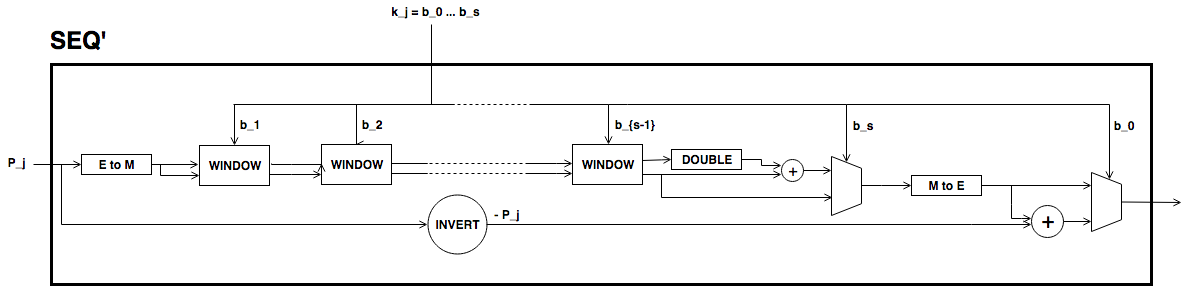
\includegraphics[scale=0.43]{figures/multiplication-SEQ-prime.png}
	\end{figure}
	
\end{enumerate}


\section{Challenges And Security}
	As required in the construction of Baby-Jubjub, the curve satisfies SafeCurves criteria. This can be checked following \cite{github-barry}.
	
\section{Implementation}	
	Barry WhiteHat:	
	\begin{itemize}
		\item %Description, generation and cryptographic requirements:
		\url{https://github.com/barryWhiteHat/baby_jubjub}
		\item %Arithmetic:
		\url{https://github.com/barryWhiteHat/baby_jubjub_ecc} 
	\end{itemize}
	Jordi Baylina: \url{https://github.com/iden3/circomlib/blob/master/src/babyjub.js}

%%	
\section {Intellectual Property}

	We will release the final version of this proposal under creative commons, to ensure it is freely available to everyone.


%% References
\addcontentsline{toc}{section}{References}
	\bibliographystyle{acm}
	\bibliography{lit}
\end{spacing}	
\end{document}
